\section{Hardware}\label{sec:hardware}
This section provides a brief overview of the hardware used in the cart pendulum setup.
\fxnote{add picture of the system (showing wires on cart)}

\subsection{Motors}
There are two Maxon 370356 brushed DC motors, see \autoref{fig:maxonMotor}, used in the setup. \fxnote{source}.

% https://www.maxonmotor.com/maxon/view/product/motor/dcmotor/re/re50/370356
\fxnote{see url source in comment}

\begin{figure}[H]
  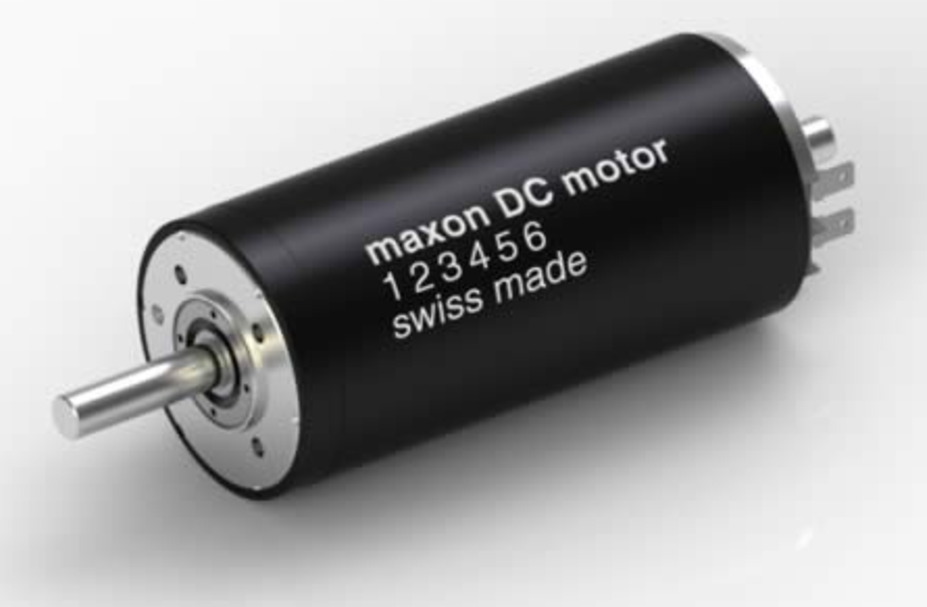
\includegraphics[width=.26\textwidth]{figures/maxonMotor}
  \caption{maxonMotor}
  \label{fig:maxonMotor}
\end{figure}

The most interesting characteristic of the maxon motor for the purposes of this report are shown in \autoref{table:motorParameters}.

\begin{table}[H]
  \begin{tabular}{|l|l|l|}
    \hline %--------------------------------------------------------------------------------------
    \textbf{Characteristic}                    & \textbf{Quantity} & \textbf{Unit}              \\
    \hline %--------------------------------------------------------------------------------------
    Nominal torque (max. continuous torque)    & \SI{420e-3}       &  \si{N \cdot m}            \\
    \hline %--------------------------------------------------------------------------------------
    Nominal current (max. continuous current)  & \SI{4.58}         &  \si{A}                    \\
    \hline %--------------------------------------------------------------------------------------
    Torque constant                            & \SI{93.4e-3}      &  \si{N\cdot m\cdot A^{-1}} \\
    \hline %--------------------------------------------------------------------------------------
    Rotor inertia                              & \SI{54.2e-6}      &  \si{kg\cdot m^2}          \\
    \hline %--------------------------------------------------------------------------------------
    Weight                                     & \SI{1.1}          &  \si{kg}                   \\
    \hline %--------------------------------------------------------------------------------------
  \end{tabular}
  \caption{'*' indicates that the parameter is estimated.\label{table:motorParameters}}
\end{table}

One of the motors is mounted on a pulley driving the belt, see \autoref{fig:systemSetup}. The other motor is disabled and acts only as a bearing at the pendulum pivot point.

\subsection{Motor Encoders}

Each of the two motors are equipped with an HEDS 5540 optical quadrature encoder, see \autoref{fig:maxonMotor}. The moment of inertia added by the encoder is negligibly small at only \SI{0.6e-6}{kg\cdot m^2} and is not mentioned further in this report.

%https://www.infineon.com/dgdl/Infineon-Encoder_HEDS-5540-A14-AP-v01_00-EN.pdf?fileId=5546d46147a9c2e40147d3d593970357
\fxnote{see url source in comment}

\begin{figure}[H]
  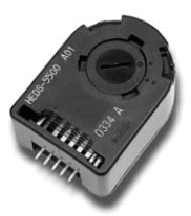
\includegraphics[width=.16\textwidth]{figures/infineonEncoderHEDS5540-A14}
  \caption{encoder}
  \label{fig:encoder}
\end{figure}

The encoder is decoded using an Avago HCTL-2021-PLC decoder which outputs 2000 ticks pr. revolution\fxnote{source} resulting in a resolution of $2\pi/2000=$ \SI{\pi e-3} rad/tic, for the pendulum angle, $\theta$, and $2\pi r /2000=2\pi\cdot 0.028 /2000\approx$ \SI{0.088e-3} m/tic for the position along $x$.

\subsection{Motor Controller}

Maxon ADS 50/10 motor controller

% https://www.maxonmotor.com/maxon/view/product/control/Servoverstaerker-4-Q-DC/201583
\fxnote{see url source in comment}

\begin{figure}[H]
  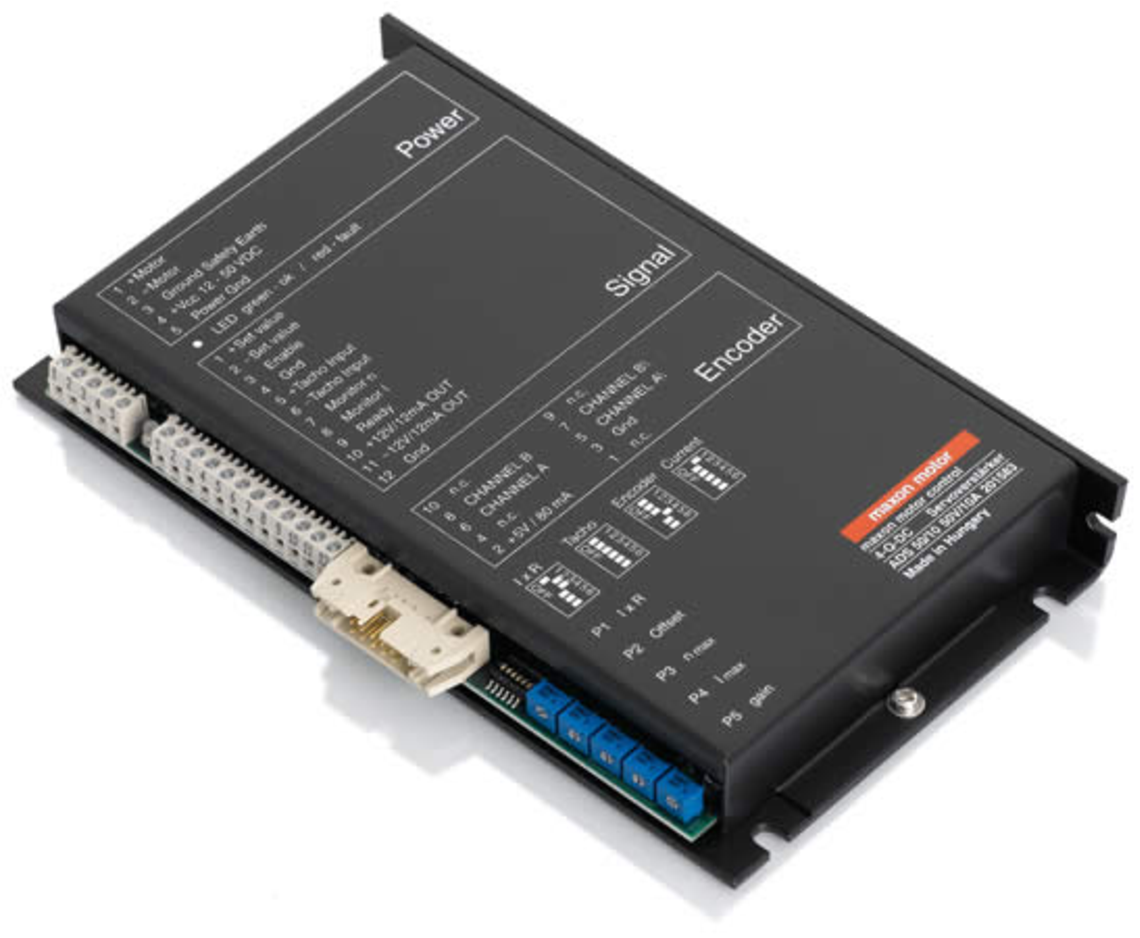
\includegraphics[width=.26\textwidth]{figures/maxonMotorController}
  \caption{maxonMotorController}
  \label{fig:maxonMotorController}
\end{figure}

\subsection{Micro Controller}

Arduino Teensy 3.6

\fxnote{source: https://www.sparkfun.com/products/14057}

\begin{figure}[H]
  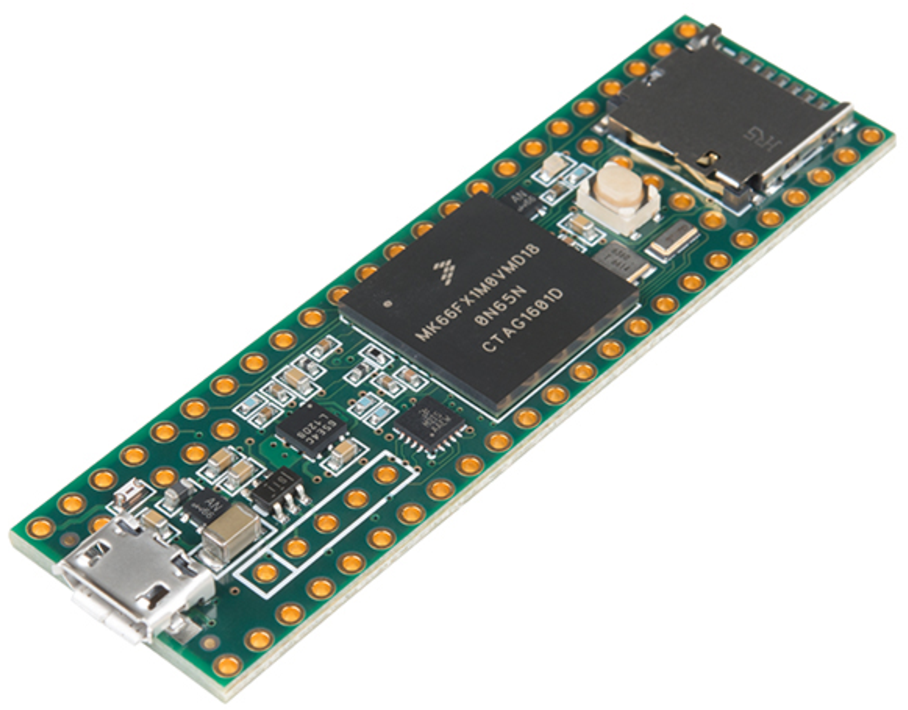
\includegraphics[width=.2\textwidth]{figures/arduinoTeensy36}
  \caption{arduinoTeensy36}
  \label{fig:arduinoTeensy36}
\end{figure}

\subsection{Shield}
Interface as described by... \fxnote{reference and at least some explanation}
